\DailyTitle{6314 Log (October 14, 2010)}

\DailySection{Goals}

\begin{enumerate}
\item Keep writing down Z candle note fragments
\item Meet with Maria to learn more about W fit
\item Start leptoquark jobs
\item Move the toy fit code to the computer and start rerunning
\item Resubmit the failed jobs
\item Keep reading Hcal DQM code
\end{enumerate}

\DailySection{Summary List}

\begin{enumerate}
\item Yay
\end{enumerate}

\DailySection{DQM code!}

An analyzer (\texttt{HcalMonitorModule}) keeps filling histograms and keeping them in memory.
The histograms (embedded in \texttt{MonitorElement}) are ``booked'' through \texttt{DQMStore} service and the ownership of the histogram memory is the service....whatever it is.
There are a list of ``clients'' that correspond to subfolders....and same story with the \texttt{DQMStore} and histogram booking.
The entrance module for the clients is \texttt{HcalMonitorClient}.  To make sure that I know what's going on,
let me introduce a new subfolder called ``HcalFHeadMonitor'' where I can put my own histograms.
Good.  Successfully installed the new subfolder.  See figure \ref{Figure_6314InstalledFHeadMonitorScreenShot}.
Try to add a histogram.  It showed up wouldn't fill at all.  Let's play with it tomorrow.

\begin{figure}
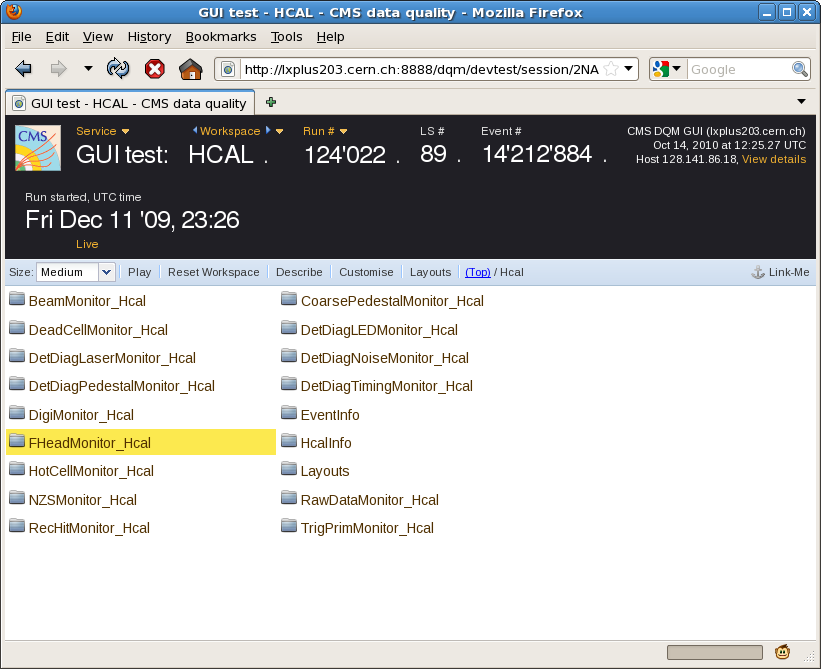
\includegraphics[width=120mm]{DailyLog/6314/6314HcalFHeadMonitor.png}
\caption{Successfully installed FHead subfolder in Hcal DQM test bench}
\label{Figure_6314InstalledFHeadMonitorScreenShot}
\end{figure}

\DailySection{Meeting about WJet simple fit}

This is the simple fit before Lukas finished with his b-tag complicated fit strategy studies.

Ilaria and somebody are going to do the fit, and I am charged to create the datasets by the end of the week.

Will showed me his code structure on making datasets.


\DailySection{Reflection}

Meow.


